\documentclass[conference]{IEEEtran}
\IEEEoverridecommandlockouts
% The preceding line is only needed to identify funding in the first footnote. If that is unneeded, please comment it out.
\usepackage{cite}
\usepackage{amsmath,amssymb,amsfonts}
\usepackage{algorithmic}
\usepackage{graphicx}
\usepackage{textcomp}
\usepackage{xcolor}
\def\BibTeX{{\rm B\kern-.05em{\sc i\kern-.025em b}\kern-.08em
    T\kern-.1667em\lower.7ex\hbox{E}\kern-.125emX}}
\begin{document}

\title{Privacy-Preserving Multi-hop Payments with Constant Collateral\\
{\footnotesize \textsuperscript{*}Note: Sub-titles are not captured in Xplore and
should not be used}
\thanks{Identify applicable funding agency here. If none, delete this.}
}

\author{\IEEEauthorblockN{1\textsuperscript{st} Given Name Surname}
\IEEEauthorblockA{\textit{dept. name of organization (of Aff.)} \\
\textit{name of organization (of Aff.)}\\
City, Country \\
email address or ORCID}
\and
\IEEEauthorblockN{2\textsuperscript{nd} Given Name Surname}
\IEEEauthorblockA{\textit{dept. name of organization (of Aff.)} \\
\textit{name of organization (of Aff.)}\\
City, Country \\
email address or ORCID}
\and
\IEEEauthorblockN{3\textsuperscript{rd} Given Name Surname}
\IEEEauthorblockA{\textit{dept. name of organization (of Aff.)} \\
\textit{name of organization (of Aff.)}\\
City, Country \\
email address or ORCID}
\and
\IEEEauthorblockN{4\textsuperscript{th} Given Name Surname}
\IEEEauthorblockA{\textit{dept. name of organization (of Aff.)} \\
\textit{name of organization (of Aff.)}\\
City, Country \\
email address or ORCID}
\and
\IEEEauthorblockN{5\textsuperscript{th} Given Name Surname}
\IEEEauthorblockA{\textit{dept. name of organization (of Aff.)} \\
\textit{name of organization (of Aff.)}\\
City, Country \\
email address or ORCID}
\and
\IEEEauthorblockN{6\textsuperscript{th} Given Name Surname}
\IEEEauthorblockA{\textit{dept. name of organization (of Aff.)} \\
\textit{name of organization (of Aff.)}\\
City, Country \\
email address or ORCID}
}

\maketitle

\begin{abstract}
This document is a model and instructions for \LaTeX.
Test for pull.
This and the IEEEtran.cls file define the components of your paper [title, text, heads, etc.]. *CRITICAL: Do Not Use Symbols, Special Characters, Footnotes, 
or Math in Paper Title or Abstract.
\end{abstract}

\begin{IEEEkeywords}
component, formatting, style, styling, insert
\end{IEEEkeywords}

\section{Introduction}
In recent years, permissionless cryptocurrencies, have emerged as a novel means to facilitate secure
and reliable payments within a decentralized framework, garnering significant attention from both academia and industry. 
These cryptocurrencies employ a consensus mechanism to verify each transaction, which is
then recorded on a publicly distributed ledger known as blockchain. Unfortunately, 
the widespread adoption of cryptocurrencies is hidered by notable scalability chanllenges. Complex consensus mechanisms, like Bitcoin's Proof-of-work(PoW), 
and the limited block size of the blockchain contribute to the issue. The theoretical
throughput of Bitcoin stands at approximately 10 transactions per second(TPS), with a transaction confirmation time of 
around 1 hour. In contrast, traditional decentralized payment networks, 
such as Visa, boast the capability up to 47,000 TPS. Furthermore, the presence of high transaction fees renders small-value 
payments impractical for cryptocurrency users.

One promising solution proposed to tackle the issue of scalability is the implements of payment channels(PCs).
PCs are off-chain payment protocols that enable two parties, who have established a channel,to conduct quick and
validated transaction off-chain. To elaborate, the overrall process can be divided into three phases. Firstly, 
during the channel-openning phase, both users commit a portion of their coins to a shared address as
initial funds, which is executed on-chain. In the subsequent channel-updating phase, the involved parties have
the flexibility to engage in numerous off-chain transactions. They can adjust the allocation of funds between themselves
by generating and exchanging signed transaction message. Ultimately, when the participants opt to settle the 
channel or encounter a dispute, they initiate the closing process by broadcasting the latest signed transaction
to the blockchain. This transaction represents the most up-to-date distribution of funds within the channel.

\section{Background}
In this section, we provide an overview on the background and the
notations used throughout the paper.
\subsection{UTXO model}

In this work, we assume the underlying blockchain, like Bitcoin, is based on the UTXO model. Transaction output is the fundamental 
component of Bitcoin transaction,which is an indivisible Bitcoin currency recorded on the blockchain and recognized as valid by 
the entire network. The Bitcoin complete nodes tracks all available outputs called \emph{unspent transaction outpus} (UTXO). 
UTXOs can be any value and once generated are indivisible, a UTXO can only be consumed as a whole in a single transaction. 
The output consists of two parts,which we represent as a tuple $\theta :=\{cash,\phi\}, \theta.cash$ is the output value,
 and the $\theta.\phi$ is the condition to spend this output, it also called \emph{locking script}. Onesig(\emph{U}) indicates 
 that the condition required to spend this output is a digital signature. We say that a user \emph{U} can spend an output only if
 $\theta.\phi$ contains only a signature w.r.t verification \emph{U}'s public key, if multiple signatures are required, we use 
 MultiSig($\it U_1,U_2,...,U_n$).

 %插图
\begin{figure}[t]
    \centering
    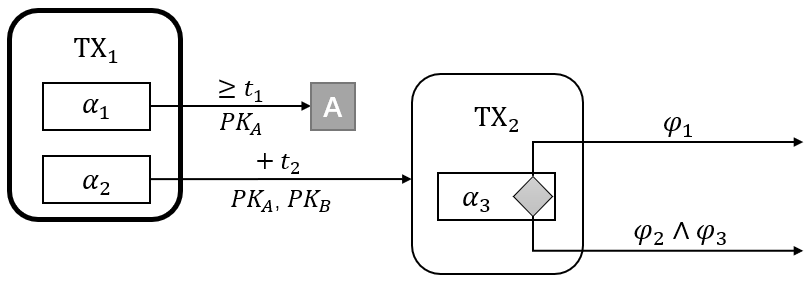
\includegraphics[scale=0.5]{fig2.png}
    \caption{Left transaction $TX_1$ is recorded on the blockchain, which has two output. Value $\alpha_1$ can spent by A, with a 
    transaction signed w.r.t $PK_A$ after $\emph{t}_1$ rounds, and the output of value $\alpha_2$ can be spent by a transaction signed w.r.t 
    $PK_A$ and $PK_B$ but only if at least $\emph{t}_2$ rounds has passed through after the transaction being published on the blockchain. The
    right transaction $TX_2$ has one input which is the second output of $TX_1$ with the value $\alpha_1$. $TX_2$ has only one
    output containing $\alpha_3$ coins, which can spent by a transaction whose witness satisfies the condition $\varphi_1 \vee (\varphi_2 
    \wedge \varphi_3)$}
\end{figure}

 Transactions consume previously recorded unused UTXOs and create new UTXOs available for future transaction, in this way, the 
 transaction continues in the form of a chain of owners. on the chain, the input of the transaction corresponds to the output 
 of the previous transaction. We denote a transaction as a tuple TX := \{id,input,output,timelock,witness\}, TX.id$\in\{0,1\}^*$
 is the identifier of a transaction and TX.id = $\mathcal H$(TX.input,TX.output,TX.timelock), $\mathcal H$ is a hash function,
 modeled as a random oracle. TX.input and TX.output denotes the list of the inputs and the list of new outputs respectively.
 $\bf TX$.timelock defined as the earliest time a transaction is valid and can be transmitted on the network or added to the blockchain, 
 it defaults to 0 in most transactions. TX.witness$\in\{0,1\}^*$, also called \emph{ScriptSig}, is part of the transaction input to address or satisfy the spending 
 conditions set by the \emph{locking script} on the output. Actually, before being recorded on the blockchain, transactions must go
 through the consensus mechanism of all nodes. During this period, each node will independently verify the transaction. For specific 
 details please refer to \colorbox{yellow}{[]}, we will only briefly describe the key parts: For a transaction(1) The sum of the input value cannot be less 
 than the sum of the output value;(1)For each input, the quoted output cannot exist in any other transaction, it must exist and not 
 be spent;(3) The \emph{ScriptSig} for each input must be validated against the \emph{locking script} for the corresponding output.
 To put it simply, the transaction must provide valid validation that satisfies the spending conditions of each input.

 We use charts to visualize the transaction for a clearer illustration. Rounded rectangles represent transactions, thick-edged rectangles 
 represent transactions that have already been published on the blockchain, and thin-edged rectangles for transactions to be published.
 The transaction contains at least one box to represent the output of the transaction, and the value in the box indicates the number of 
 coins in this output. On the arrows coming from the output, are noted the conditions under which this output is spent. The public key 
 below the arrow indicates who can use this output; Above the arrow is the timelock for the output(in this work only uses timelock 
 as additional condition, which in practice could be any script supported by the underlying blockchain scripting language). There are 
 two types of timelocks: \emph{relative time lock} and \emph{absolute time lock}, we use "+\emph{t}" to represent the relative time lock, 
 that is, the transaction only vaild at least \emph{t} blocks has passed through after the transaction being recorded on the blockchain; 
 The absolute time lock "$\geq$\emph{t}" specifies the absolute time point, indicating that the first transaction has passed through \emph{t} 
 round after being recorded on the blockchain. Finally, we use a diamond to represent the relationship of "or" that the output conditions are 
 different, expressed in the symbolic form as $\varphi = \varphi_1 \vee ...\vee \varphi_n$, where $\varphi$ is the output locking script,
 written on the arrows of the output. A complete example is given in Fig. \colorbox{yellow}{1}.


\subsection{Payment channels}

The payment channel is opened by two users locking some coins on the blockchain, and then the two parties can make as many quick 
instant confirmation transactions off-chain, that is, without waiting for transmitting the transaction to the blockchain, as long 
as the total amount of each transaction is less than the locked value. During the lifetime of the channel, only two transactions 
will be recorded on the blockchain, one is funding transaction $TX_f$ which used to open the channel, the other is settlement 
transaction for close the channel. The funding transaction $TX_f$ determines the balance of this channel, and the channel is open 
when $TX_f$ is broadcast to the network and recorded on the blockchain, both parties update the channel balance by exchanging signed 
transactions off-chain, these transactions holding the reassigned balances are called state of the channel $TX_{state}$. Finally, the 
channel is closed by posting settlement transaction, which is the final state, on the blockchain.In a more detil, there are three 
operations of the payment channel: $\emph{open, update,}$ and  $\emph{close}$.

1) \emph{Open}

\subsection{Payment channel networks}

The IEEEtran class file is used to format your paper and style the text. All margins, 
column widths, line spaces, and text fonts are prescribed; please do not 
alter them. You may note peculiarities. For example, the head margin
measures proportionately more than is customary. This measurement 
and others are deliberate, using specifications that anticipate your paper 
as one part of the entire proceedings, and not as an independent document. 
Please do not revise any of the current designations.

\section{Solution Overview}
In this section, we present our key idea.

\subsection{Security and privacy goals}

Define abbreviations and acronyms the first time they are used in the text, 
even after they have been defined in the abstract. Abbreviations such as 
IEEE, SI, MKS, CGS, ac, dc, and rms do not have to be defined. Do not use 
abbreviations in the title or heads unless they are unavoidable.

\subsection{Key idea}

Define abbreviations and acronyms the first time they are used in the text, 
even after they have been defined in the abstract. Abbreviations such as 
IEEE, SI, MKS, CGS, ac, dc, and rms do not have to be defined. Do not use 
abbreviations in the title or heads unless they are unavoidable.

\section{Constrution}

\subsection{Building blocks}

Define abbreviations and acronyms the first time they are used in the text, 
even after they have been defined in the abstract. Abbreviations such as 
IEEE, SI, MKS, CGS, ac, dc, and rms do not have to be defined. Do not use 
abbreviations in the title or heads unless they are unavoidable.

\subsection{Protocol description}

Define abbreviations and acronyms the first time they are used in the text, 
even after they have been defined in the abstract. Abbreviations such as 
IEEE, SI, MKS, CGS, ac, dc, and rms do not have to be defined. Do not use 
abbreviations in the title or heads unless they are unavoidable.

\section{Analysis}

\subsection{Security}

Define abbreviations and acronyms the first time they are used in the text, 
even after they have been defined in the abstract. Abbreviations such as 
IEEE, SI, MKS, CGS, ac, dc, and rms do not have to be defined. Do not use 
abbreviations in the title or heads unless they are unavoidable.

\subsection{High level functionality description}

Define abbreviations and acronyms the first time they are used in the text, 
even after they have been defined in the abstract. Abbreviations such as 
IEEE, SI, MKS, CGS, ac, dc, and rms do not have to be defined. Do not use 
abbreviations in the title or heads unless they are unavoidable.

\section{Evaluation}

The implementtion and evaluation.

\section{Discussion}

Some arguements

\section{Conclution}

Conclude the paper.

\section*{References}

Please number citations consecutively within brackets \cite{b1}. The 
sentence punctuation follows the bracket \cite{b2}. Refer simply to the reference 
number, as in \cite{b3}---do not use ``Ref. \cite{b3}'' or ``reference \cite{b3}'' except at 
the beginning of a sentence: ``Reference \cite{b3} was the first $\ldots$''

Number footnotes separately in superscripts. Place the actual footnote at 
the bottom of the column in which it was cited. Do not put footnotes in the 
abstract or reference list. Use letters for table footnotes.

Unless there are six authors or more give all authors' names; do not use 
``et al.''. Papers that have not been published, even if they have been 
submitted for publication, should be cited as ``unpublished'' \cite{b4}. Papers 
that have been accepted for publication should be cited as ``in press'' \cite{b5}. 
Capitalize only the first word in a paper title, except for proper nouns and 
element symbols.

For papers published in translation journals, please give the English.
citation first, followed by the original foreign-language citation \cite{b6}.

\begin{thebibliography}{99}
\bibitem{b1} G. Eason, B. Noble, and I. N. Sneddon, ``On certain integrals of Lipschitz-Hankel type involving products of Bessel functions,'' Phil. Trans. Roy. Soc. London, vol. A247, pp. 529--551, April 1955.
\bibitem{b2} J. Clerk Maxwell, A Treatise on Electricity and Magnetism, 3rd ed., vol. 2. Oxford: Clarendon, 1892, pp.68--73.
\bibitem{b3} I. S. Jacobs and C. P. Bean, ``Fine particles, thin films and exchange anisotropy,'' in Magnetism, vol. III, G. T. Rado and H. Suhl, Eds. New York: Academic, 1963, pp. 271--350.
\bibitem{b4} K. Elissa, ``Title of paper if known,'' unpublished.
\bibitem{b5} R. Nicole, ``Title of paper with only first word capitalized,'' J. Name Stand. Abbrev., in press.
\bibitem{b6} Y. Yorozu, M. Hirano, K. Oka, and Y. Tagawa, ``Electron spectroscopy studies on magneto-optical media and plastic substrate interface,'' IEEE Transl. J. Magn. Japan, vol. 2, pp. 740--741, August 1987 [Digests 9th Annual Conf. Magnetics Japan, p. 301, 1982].
\bibitem{b7} M. Young, The Technical Writer's Handbook. Mill Valley, CA: University Science, 1989.
\end{thebibliography}
\vspace{12pt}
\color{red}
IEEE conference templates contain guidance text for composing and formatting conference papers. Please ensure that all template text is removed from your conference paper prior to submission to the conference. Failure to remove the template text from your paper may result in your paper not being published.

\end{document}
